
% This LaTeX was auto-generated from MATLAB code.
% To make changes, update the MATLAB code and republish this document.

\documentclass{article}
\usepackage{graphicx}
\usepackage{color}

\sloppy
\definecolor{lightgray}{gray}{0.5}
\setlength{\parindent}{0pt}

\begin{document}

    
    \begin{verbatim}
%%%%%% Disretising the Boundary Integral Equation for the equation
%%%%%% lap(u) + k^2u = 0     on the domain B(0,1)
%%%%%% u = f       on the boundary of B(0,1)
clear;

%%%%%%%%%%%       Trapezoidal Rule for sin(x^2log(|x|))       %%%%%%%%%%%%%
%
f = @(x) (x.^2).*log(abs(x));
% f = @(x) x.*log(abs(x));
a = -1; b = 1;
nn = 1001;
ns = 1:2:nn;
I = zeros(length(ns),1);
for i = 1:length(ns)
    h = (b-a)/ns(i);
    l = [1/2; ones(ns(i)-1,1); 1/2];
    v = a:h:b;
    I(i) = h * f(v) * l;
end
p = 7001;
hh = (b-a)/p;
ll = [1/2; ones(p-1,1); 1/2];
vv = a : hh : b;
inte1 = hh * f(vv) * ll;
inte = integral(@(x) f(x), a, b);
loglog(ns, abs(I-inte), 'r.', 'MarkerSize', 15);
hold on; loglog(ns, 0.5*ns.^(-2), 'b.', 'MarkerSize', 10);

return
%%%%%%%% Definition of function and the boundary  %%%%%%%%%%

x0 = [5.1 3.14];
k = 1;
f = @(x) (1j/4)*besselh(0, k * sqrt( (x(:,1) - x0(:,1)).^2 + (x(:,2) - x0(:,2)).^2 ) );
a = 0.4; m = 3; b = 2;

% ge = @(t) [a*cos(t);b*sin(t)];
% der_ge = @(x) [-a*sin(x); b*cos(x)];
% der2_ge = @(x) [-a*cos(x); -b*sin(x)];
% nge = @(t) [b*cos(t);a*sin(t)]./( ((b*cos(t)).^2 + (a*sin(t)).^2).^0.5 );

ge = @(t) (1 + a*cos(m*t)).*[cos(t);sin(t)];
der_ge = @(t) -a*m*sin(m*t).*[cos(t);sin(t)] + (1 + a*cos(m*t)).*[-sin(t);cos(t)];
der2_ge = @(t) -(1 + a*cos(m*t)).*[cos(t);sin(t)] + 2*a*m*sin(m*t).*[sin(t);-cos(t)]...
            -a*m*m*cos(m*t).*[cos(t);sin(t)];
speed =  @(t) -a*m*sin(m*t).*[sin(t);-cos(t)] + (1 + a*cos(m*t)).*[cos(t);sin(t)];
nge = @(t) speed(t)./vecnorm(speed(t));


%%%%  Defn of pts where diff betweenn true sol and double_layer is evaluated  %%%%

jj = 100;
pp = -pi : pi/jj : pi;
dir = [cos(pp);sin(pp)].';
rng(1);                                    %%%%%% random number generator fixes seed
rr = 0.5 * min(a,b) * rand(length(pp),1);
x = rr.*dir;
xp = x(:,1); yp = x(:,2);

%%%%% Defn of true sol  %%%%%%%

sol = f(x);



    % n = 500;
    % t = -2*pi*n/(2*n+1) : 2*pi/(2*n+1) : pi;
    %
    % %%% Calculating bdry pts and bdry normal  %%%%
    % xx = ge(t).';
    % nxx = nge(t).';
    % w = (2*pi)/(2*n+1);   % weight associated with the parameterisation
    % l = length(xx(:,1));
    % y = f(xx);           % y for f = log|x-x0|   or   f = 5
    % absder_g = (((der_ge(t).').^2)*[1;1]).^(0.5);
    % ker = get_kerneldl(k, t, ge, nge, der_ge, der2_ge);
    % A = -0.5*eye(2*n+1) + w*ker.*(absder_g.');
    % sigma = A\y;



% n = 100;
% t = -2*pi*n/(2*n+1) : 2*pi/(2*n+1) : pi;

%%%% Calculating bdry pts and bdry normal for sigma evaluation  %%%%
% xx = ge(t).';
% nxx = nge(t).';
%
% l = length(xx(:,1));
% y = f(xx);           % y for f = log|x-x0|   or   f = 5
% w = (2*pi)/(2*n+1);
% absder_g = (((der_ge(t).').^2)*[1;1]).^(0.5);
% ker = get_kerneldl(k, t, ge, nge, der_ge, der2_ge);
% A = -0.5*eye(2*n+1) + w*ker.*(absder_g.');
% sigma = A\y;
% xg = xx(:,1).'; yg = xx(:,2).';
% xn = nxx(:,1).'; yn = nxx(:,2).';
% xgm = repmat(xg, length(xp), 1);
% ygm = repmat(yg, length(yp), 1);

%%%%%  Calculation of Sigma %%%%%%
ns = 1:25:1000;
err = zeros(length(ns), 1);
for ii = 1:length(ns)
    n = ns(ii);
    % n = 100;
    t = -2*pi*n/(2*n+1) : 2*pi/(2*n+1) : pi;

    %%%% Calculating bdry pts and bdry normal  %%%%
    xx = ge(t).';
    nxx = nge(t).';
    w = (2*pi)/(2*n+1);         % weight associated with the parameterisation
    l = length(xx(:,1));
    y = f(xx);                  % y for f = log|x-x0|   or   f = 5
    absder_g = (((der_ge(t).').^2)*[1;1]).^(0.5);
    ker = get_kerneldl(k, t, ge, nge, der_ge, der2_ge);
    A = -0.5*eye(2*n+1) + w*ker.*(absder_g.');
    sigma = A\y;


    % jj = 100;
    % pp = -pi:pi/jj:pi;
    % dir = [cos(pp);sin(pp)].';
    % rng(1);                                    %%%%%% random number generator fixes seed
    % rr = (ii/length(ns)) * min(a,b) * rand(length(pp),1);
    % x = rr.*dir;
    % xp = x(:,1); yp = x(:,2);
    %
    % %%%% Defn of true sol  %%%%%%%
    %
    % sol = f(x);

    %%%%%%% Calculating Double Layer %%%%%%%


    xg = xx(:,1).'; yg = xx(:,2).';
    xn = nxx(:,1).'; yn = nxx(:,2).';
    xgm = repmat(xg, length(xp), 1);
    ygm = repmat(yg, length(yp), 1);
    xpt = repmat(xp, 1, length(xg));
    ypt = repmat(yp, 1, length(yg));
    double_layer = (1i*k*w/4)*( besselh(1, k*sqrt( (xpt - xgm).^2 + ...
                        (ypt - ygm).^2)).*( (xpt - xgm).*xn + (ypt - ygm).*yn )./ ...
                        (sqrt( (xpt - xgm).^2 + (ypt - ygm).^2) ) )*(sigma.*absder_g);


    %%%%%%%%%% Calculating error between true sol and Double Layer %%%%%%%%%

    err(ii) = max(abs(sol - double_layer));
end
figure; loglog(ns, err, 'r.', 'MarkerSize', 10);
% hold on; semilogy(ns, exp(-0.3*ns), 'b.')




function [ker] = get_kerneldl(k, t, gamma, normal, der1, der2)
x = gamma(t).';
n = normal(t).';
d1 = der1(t).';
d2 = der2(t).';
xx = x(:,1); xy = x(:,2);
nx = n(:,1).'; ny = n(:,2).';
xpt = repmat(xx, 1, length(xx)); xgm = repmat(xx.', length(xx), 1);
ypt = repmat(xy, 1, length(xy)); ygm = repmat(xy.', length(xy), 1);

ker = (1i*k/4)*besselh(1,k*sqrt( (xpt-xgm).^2 + (ypt-ygm).^2)) .*((xpt-xgm).*nx ...
            + (ypt-ygm).*ny)./(sqrt( (xpt-xgm).^2 + (ypt-ygm).^2));

for i = 1:length(ker(:,1))
    ker(i,i) = (1/(4*pi))*( n(i,1)*d2(i,1) + n(i,2)*d2(i,2) )/(  d1(i,1)^2 + d1(i,2)^2  );
end
end








%%%%%%%%%%%    Learning points
% if your discretising points on "boundary" are all distant 'h' away from each other,
% then you can get the error around points in the "domain" which are at atmost
% distance 5h from the boundary.


%%%%%%%%   Homeworks %%%%%%
% 1. Plot the error as a function of the number 'n' and try to get the error
%    and try to justify it.
%   ANSWER:- For a fixed x(according to our notations which is the pts inside domain
%            where we evaluate the error), the error behaves as the
%            c.n^(-3) where c = 0.009
%            depends upon distance between the boundary and x, as the kernel
%            is of the order 1/(x-y) when x is in domain and y is in boundary.


% 2. Now try to solve the Helmholtz equation and see the asymptotics of
%    Single Layer and Double Layer in this case, where Green's function is
%    given by G(x,y) = i/4*Hankel(0,1)(k|x-y|), i.e., calculate the limit as x
%    goes to y of G_s(x,y) and limit as x goes to y of G_d(x,y)
%   ANSWER:- Look at the notes titled NODES exercise section

% 3. Plot the error in Helmholtz case and get the rates and explain the reason
%    for the deacys.
%   ANSWER:- Error is of the order

%%%%%%%   Observations %%%%%%
% 1. In this case, error is given by err(n) = c.n^(-3), which we have observed
%    by fixing the pts(x in our notations), where error is to be evaluated,
%    and varying the nodes.
% 2. In this case, also error depends on the distance of interior points and
%    boundary points, which is the "5h rule" which we have observed by fixing
%    the node as 100, and varying the distance of pts(x in our notations),
%    where error is to be evaluated, from the boundary
% 3. The nearer the points(x in our notations), where we are evaluating the
%    difference (u(x) - double_layer(x)), the more the error, which is
%    basically the point number 2
\end{verbatim}

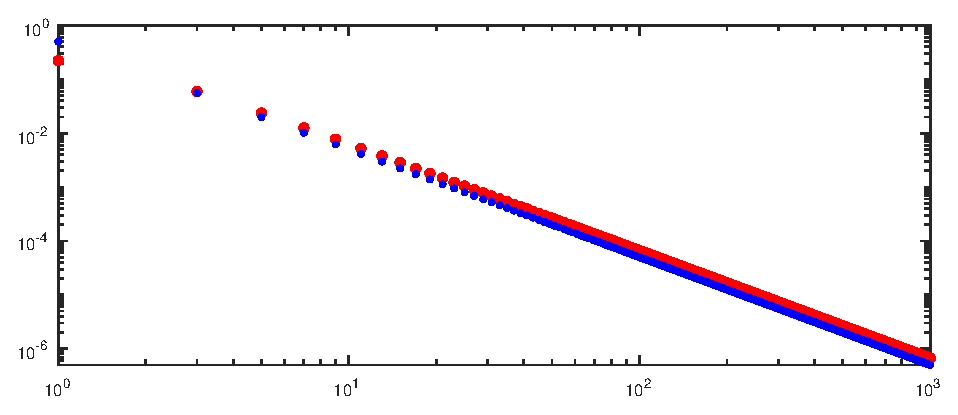
\includegraphics [width=4in]{ex_manas_helm_01.eps}



\end{document}

